Ist die Sprache
\[
L = \{\texttt{0}^i\texttt{1}^j\texttt{0}^i\mid j\le i\}
\]
kontextfrei?
Wenn ja geben Sie einen Stackautomaten an, der $L$ akzeptiert.

\thema{kontextfrei}
\themaL{Pumping Lemma fur kontextfreie Sprachen}{Pumping Lemma für kontextfreie Sprachen}

\begin{loesung}
\begin{enumerate}
\item Annahme: $L$ ist kontextfrei.
\item Gemäss Pumping Lemma für kontextfreie Sprachen gibt es die
Pumping Length $N$
\item Wähle das Wort $\texttt{0}^N\texttt{1}^N\texttt{0}^N$
\item Es lässt sich in fünf Teile $w=xyzuv$ zerlegen,
wobei $|yzu|\le N$ und $|yu|>0$ sein muss.
\begin{center}
\definecolor{darkgreen}{rgb}{0,0.6,0}
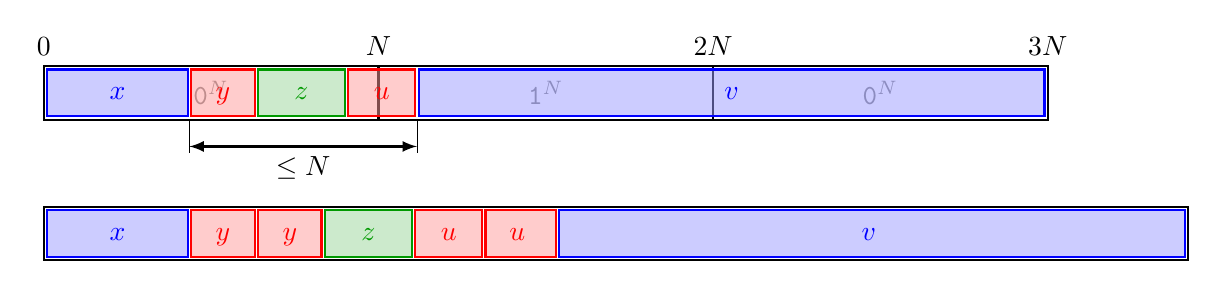
\begin{tikzpicture}[>=latex,thick,scale=0.85]

\draw (0,0) rectangle (5,0.8);
\draw (5,0) rectangle (10,0.8);
\draw (10,0) rectangle (15,0.8);

\node at (0,0.8) [above] {$0$};
\node at (5,0.8) [above] {$N$};
\node at (10,0.8) [above] {$2N$};
\node at (15,0.8) [above] {$3N$};

\node[color=gray] at (2.5,0.4) {$\texttt{0}^N$};
\node[color=gray] at (7.5,0.4) {$\texttt{1}^N$};
\node[color=gray] at (12.5,0.4) {$\texttt{0}^N$};

\fill[color=blue!40,opacity=0.5] (0.05,0.05) rectangle (2.15,0.75);
\draw[color=blue] (0.05,0.05) rectangle (2.15,0.75);
\node[color=blue] at (1.1,0.4) {$x$\strut};

\fill[color=red!40,opacity=0.5] (2.20,0.05) rectangle (3.15,0.75);
\draw[color=red] (2.20,0.05) rectangle (3.15,0.75);
\node[color=red] at (2.675,0.4) {$y$\strut};

\fill[color=darkgreen!40,opacity=0.5] (3.20,0.05) rectangle (4.50,0.75);
\draw[color=darkgreen] (3.20,0.05) rectangle (4.50,0.75);
\node[color=darkgreen] at (3.85,0.4) {$z$\strut};

\fill[color=red!40,opacity=0.5] (4.55,0.05) rectangle (5.55,0.75);
\draw[color=red] (4.55,0.05) rectangle (5.55,0.75);
\node[color=red] at (5.05,0.4) {$u$\strut};

\fill[color=blue!40,opacity=0.5] (5.60,0.05) rectangle (14.95,0.75);
\draw[color=blue] (5.60,0.05) rectangle (14.95,0.75);
\node[color=blue] at (10.275,0.4) {$v$\strut};

\draw[line width=0.3pt] (2.175,0) -- (2.175,-0.5);
\draw[line width=0.3pt] (5.575,0) -- (5.575,-0.5);
\draw[<->] (2.175,-0.4) -- (5.575,-0.4);
\node at (3.875,-0.4) [below] {$\le N$};

\begin{scope}[yshift=-2.1cm]
\draw (0,0) rectangle (17.1,0.8);

\fill[color=blue!40,opacity=0.5] (0.05,0.05) rectangle (2.15,0.75);
\draw[color=blue] (0.05,0.05) rectangle (2.15,0.75);
\node[color=blue] at (1.1,0.4) {$x$\strut};

\fill[color=red!40,opacity=0.5] (2.20,0.05) rectangle (3.15,0.75);
\draw[color=red] (2.20,0.05) rectangle (3.15,0.75);
\node[color=red] at (2.675,0.4) {$y$\strut};

\fill[color=red!40,opacity=0.5] (3.20,0.05) rectangle (4.15,0.75);
\draw[color=red] (3.20,0.05) rectangle (4.15,0.75);
\node[color=red] at (3.675,0.4) {$y$\strut};

\fill[color=darkgreen!40,opacity=0.5] (4.20,0.05) rectangle (5.50,0.75);
\draw[color=darkgreen] (4.20,0.05) rectangle (5.50,0.75);
\node[color=darkgreen] at (4.85,0.4) {$z$\strut};

\fill[color=red!40,opacity=0.5] (5.55,0.05) rectangle (6.55,0.75);
\draw[color=red] (5.55,0.05) rectangle (6.55,0.75);
\node[color=red] at (6.05,0.4) {$u$\strut};

\fill[color=red!40,opacity=0.5] (6.60,0.05) rectangle (7.65,0.75);
\draw[color=red] (6.60,0.05) rectangle (7.65,0.75);
\node[color=red] at (7.075,0.4) {$u$\strut};

\fill[color=blue!40,opacity=0.5] (7.70,0.05) rectangle (17.05,0.75);
\draw[color=blue] (7.70,0.05) rectangle (17.05,0.75);
\node[color=blue] at (12.325,0.4) {$v$\strut};

\end{scope}


\end{tikzpicture}
\end{center}
\item Da $|yzu|\le N$ kann $yzu$ nur Nullen aus einem der beiden Nullenblöcke
enthalten.
Beim Pumpen nimmt die Zahl der Nullen im betroffenen Block zu, jedoch nicht
im anderen, das gepumpte Wort liegt daher nicht mehr in der Sprache.

Es gibt noch eine zweite Situation, die beim Pumpen eintreten könnte.
Es könnten in $y$ und $u$ nur Einsen haben.
In diesem Fall würde aber beim Pumpen die Zahl der Einsen zunehmen.
Nach genügend vielen Pump-Schritten wäre die Anzahl der Einsen grösser
als die Zahl $N$ der Nullen.
Damit wäre das gempumpte Wort wieder nicht länger in der Sprache,
im Widerspruch zur Aussage des Pumping Lemma.
\item Aus dem Widerspruch kann geschlossen werden, dass die Sprache
$L$ nicht kontextfrei sein kann.
\qedhere
\end{enumerate}
\end{loesung}

\begin{bewertung}
Annahme kontextfrei ({\bf PL}) 1 Punkt,
Pumping Length $N$ ({\bf N}) 1 Punkt,
Wahl eines geeigneten Wortes ({\bf W}) 1 Punkt,
Aufteilung in 5 Teile {(\bf A)} 1 Punkt,
Widerspruch beim Pumpen ({\bf W)} 1 Punkt,
Schlussfolgerung ({\bf S}) 1 Punkt.
\end{bewertung}
